% This is samplepaper.tex, a sample chapter demonstrating the
% LLNCS macro package for Springer Computer Science proceedings;
% Version 2.20 of 2017/10/04
%
\documentclass[runningheads]{llncs}
%
\usepackage{graphicx}
% Used for displaying a sample figure. If possible, figure files should
% be included in EPS format.
%


\graphicspath{ {figuras/} }

\usepackage{float}
\usepackage{longtable}
\usepackage{listings}
\usepackage{amsmath}
\usepackage{systeme}
\usepackage{csquotes}
\usepackage{hyperref}
\hypersetup{
    colorlinks=true, %set true if you want colored links
    linktoc=all,     %set to all if you want both sections and subsections linked
    linkcolor=blue,  %choose some color if you want links to stand out
}
% If you use the hyperref package, please uncomment the following line
% to display URLs in blue roman font according to Springer's eBook style:
\renewcommand\UrlFont{\color{blue}\rmfamily}
% The amsmath package provides a handful of options for displaying equations. You can choose the layout that better suits your document, even if the equations are really long, or if you have to include several equations in the same line.

%encoding
%--------------------------------------
\usepackage[T1]{fontenc}
\usepackage[utf8]{inputenc}
%--------------------------------------
%Portuguese-specific commands
%--------------------------------------
\usepackage[portuguese]{babel}
%--------------------------------------
%Hyphenation rules
%--------------------------------------
\usepackage{hyphenat}
\hyphenation{mate-mática recu-perar ma-no equa-ções}

\begin{document}
%
\title{Obtenção de instâncias e resoluções de puzzles do Problema de Decisão Gold Star}
%
\titlerunning{Solução de Puzzles Gold Star}
% If the paper title is too long for the running head, you can set
% an abbreviated paper title here
%
\author{André Gomes\orcidID{up201806224} e
Gonçalo Teixeira\orcidID{up201806562}}
%
\authorrunning{Gonçalo Teixeira e André Gomes}
% First names are abbreviated in the running head.
% If there are more than two authors, 'et al.' is used.
%
\institute{FEUP-PLOG, Turma 3MIEIC06, Grupo Gold\_Star\_4 \\
\url{http://web.fe.up.pt}}
%
\maketitle              % typeset the header of the contribution
%
\begin{abstract}
% Requested
Começa-se por definir o objetivo deste projeto na Introdução, seguido de uma breve informação sobre cada ponto do relatório. Na descrição do problema explica-se em que é que consiste o puzzle Gold Star e como este se simplifica num sistema de equações. Na abordagem explicita-se as variáveis de decisão deste PSR juntamente com as restrições aplicadas aos operadores e ás variáveis de resultado. Esta secção é seguida de uma breve demonstração de como é feita a visualização das soluções, em formato estrela e em formato de lista, antes da maior secção, as experiências realizadas. São primeiro demonstrados os resultados da análise dimensional e como o tempo de execução cresce exponencialmente com a complexidade da estrela, seguido pela análise de estratégias de pesquisa, nomeadamente os melhores argumentos usados no labeling. Terminando o relatório com uma conclusão e possível trabalho futuro.

\keywords{Configuração  \and Operadores \and Gold Star}
\end{abstract}
%
%
%
\section{Introdução}
% Requested

Este relatório detalha o projeto desenvolvido para o segundo trabalho prático da unidade curricular de Programação em Lógica do MIEIC-FEUP, na qual se explora o puzzle Gold Star e como este pode ser resolvido com auxilio a programação em lógica por restrições. O objetivo inicial proposto para este trabalho foi de criar um ficheiro que contenha todas as soluções possíveis do puzzle Gold Star, partindo de uma estrela de cinco pontas. Não sabendo o grau de exigência computacional que este problema poderia ou não ter, tornou-se um desafio interessante da qual conseguimos retirar conclusões satisfatórias.

O relatório começa por descrever o problema estudado, passando para a abordagem tomada por nós para o resolver, contendo detalhes sobre as variáveis de decisão usadas e as restrições aplicadas. Após isto é brevemente mencionado como é feita a representação dos problemas e soluções, acabando com uma análise das experiências executadas, junto com as conclusões possíveis de retirar dos dados obtidos.

\section{Descrição do Problema}
% Requested

O problema de decisão Gold Star consiste em resolver um sistema de 5 equações da forma
\begin{equation}
\systeme*{
A \_ B = D \_ E ,
G \_ F = D \_ C ,
I \_ H = F \_ E ,
G \_ H = J \_ A ,
I \_ J = B \_ C
}
\end{equation}
Sendo \_ possível de ser substituído por um dos seguintes operadores:
\begin{equation}
    +\  -\  \mbox{×}\ \ \mbox{÷}
\end{equation}

Entre as 5 equações, apenas são partilhadas 10 variáveis para ser possível formar um padrão em forma de estrela ao dispor as equações como na figura \ref{fig: gold_star_example}.

\begin{figure}[ht]
\centering
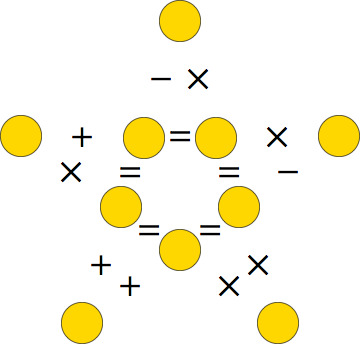
\includegraphics[width=0.3\textwidth]{figuras/template.jpg}
\caption{5 equações dispostas em padrão de forma estrela}
\label{fig: gold_star_example}
\end{figure}

Para obter uma solução válida, apenas podem ser usados os números inteiros de 0 até 9 e cada dígito só pode ser usado uma vez. Para além disso, os resultados de cada lado da equação não podem resultar em números não inteiros.

\section{Abordagem}
% Requested

Os puzzles Gold Star correspondem a um problema de decisão, ou um problema de satisfação de restrições - \textbf{PSR}. Por isso, nos próximos 2 pontos são explicadas as variáveis usadas, tal como os seus domínios, e as restrições aplicadas que restringem os valores das variáveis dentro dos seus domínios.
\subsection{Variáveis de Decisão}
% Requested

Tendo como ponto de partida uma configuração do problema Gold Star como a da Fig.\ref{fig: gold_star_example}, é possível obter uma lista de operadores que servem como argumento para o predicado \verb|gold_star/2|.

O predicado \verb|gold_star/2|, a partir de uma lista de operadores, consegue calcular uma solução para uma configuração, usando programação em lógica com restrições. Este predicado possui dez variáveis de decisão, uma para cada variável do sistema de equações, guardadas numa Lista \verb|Result|, cujo domínio é \verb|[0,9]|.

Para obter configurações do problema temos o predicado \verb|operators/3|, que faz uso de restrições para criar configurações dos operadores do problema. Este predicado possui também 10 variáveis de decisão, cada uma correspondendo a um operador. O domínio é \verb|[1,4]|, para que cada operador corresponda a um número inteiro, de acordo com os predicados \verb|numb_signal/2|.

\subsection{Restrições}
% Requested

Devido à simplicidade do problema, este não contém restrições flexíveis, apenas restrições rígidas, tanto para os operadores como para os operandos.

% -----------------

\subsubsection{Operadores} No predicado \verb|operators(1,_,_)| é criada uma lista de operadores que pode ser alimentada ao predicado \verb|gold_star/2|. Nesta criação é aplicada uma restrição explicita no predicado \verb|bigger/2|:

\begin{proof}
O primeiro operador de uma configuração deve ter maior ou igual valor numérico que os restantes operadores
\end{proof}

\begin{figure}[h]
\centering
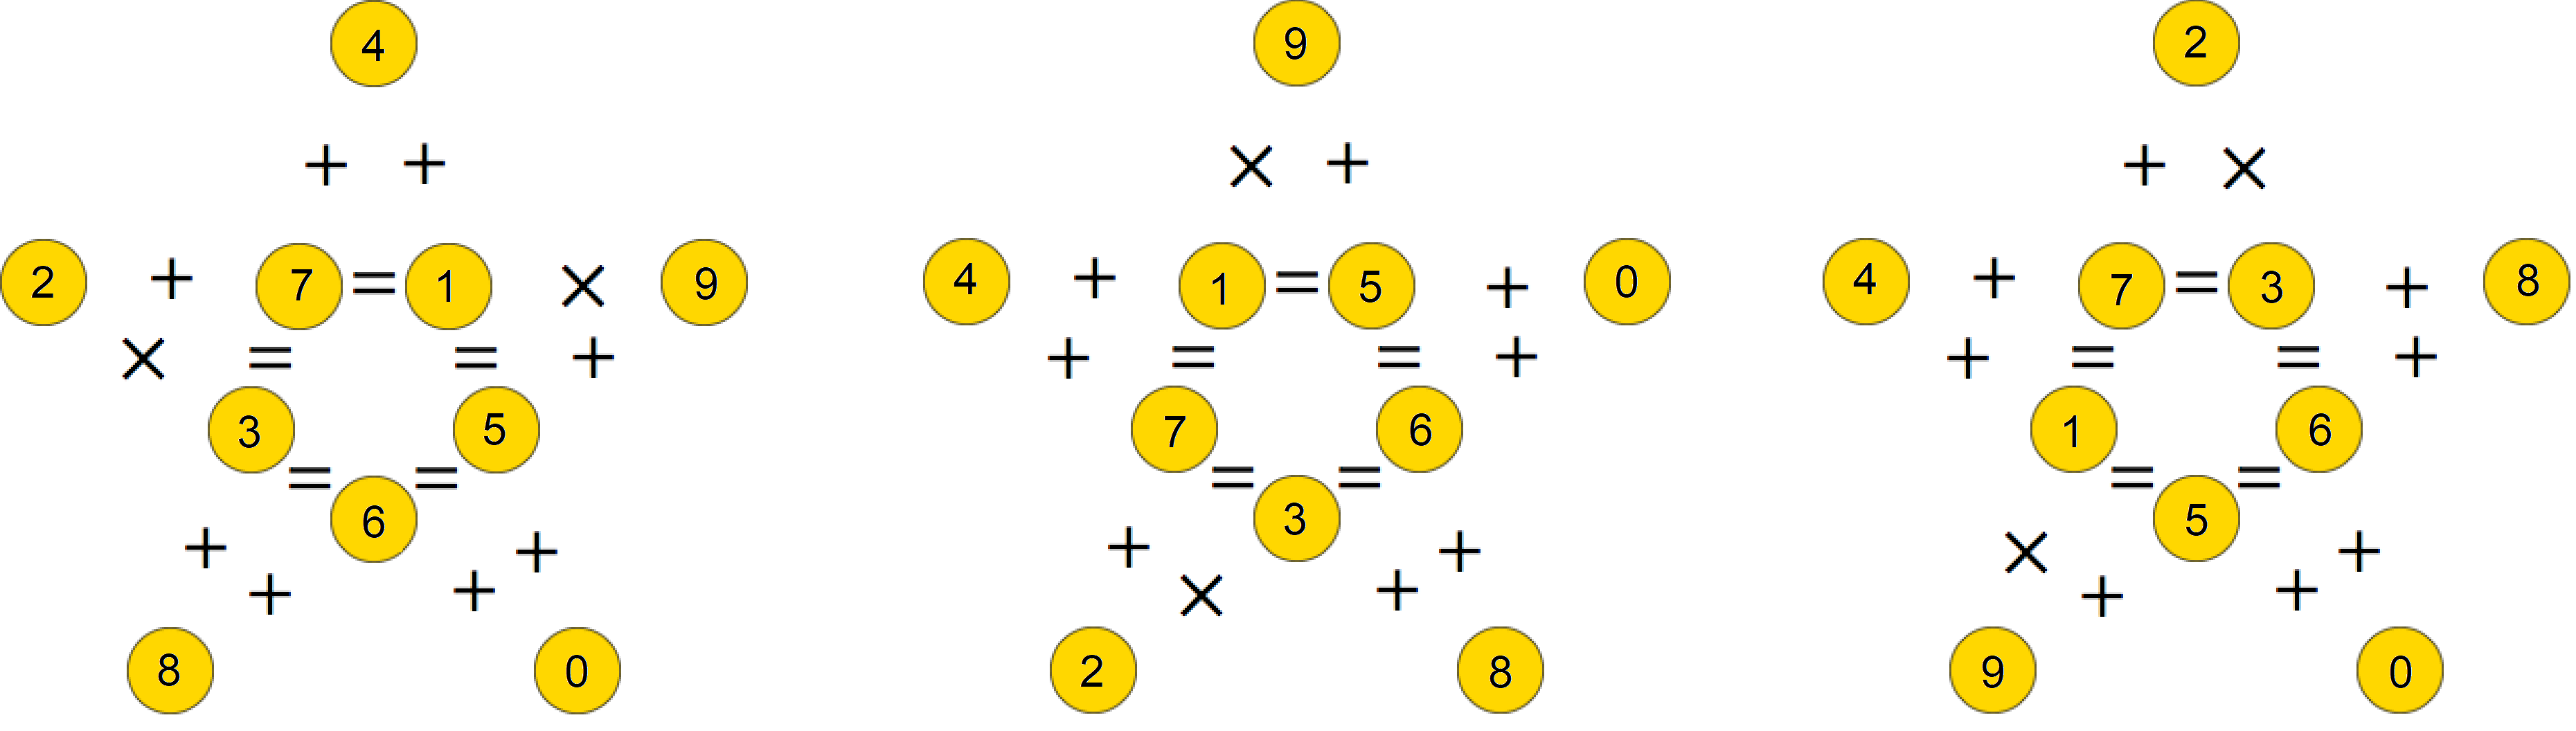
\includegraphics[width=\textwidth]{figuras/rotated.png}
\caption{A estrela do centro tem a configuração [3,1,1,1,1,1,3,1,1,1]. A estrela da esquerda é obtida através de uma rotação da estrela do centro, formando a configuração [1,1,3,1,1,1,1,1,3,1]. A estrela da direita é obtida através de uma combinação de uma rotação e uma reflexão, resultando na configuração [1,3,1,1,1,1,1,3,1,1]}
\label{fig: ops_restriction}
\end{figure}

Na figura \ref{fig: ops_restriction} apenas a configuração central obedece à restrição e só essa configuração é calculada. Todas as outras configurações, possíveis de obter através de deslocamentos de todos os elementos dentro da lista correspondem a aplicar rotações e reflexões na estrela original, o que faz com que seja desnecessário calcular estas configurações, já que são facilmente obtidas.

\begin{figure}
    \centering
    \begin{tabular}{c}
    \begin{lstlisting}[language=Prolog]
    bigger(_, []).
    bigger(Op1, [Op | Rest]) :-
        Op1 #>= Op,
        bigger(Op1, Rest).
    \end{lstlisting}
    \end{tabular}
    \caption{Predicado bigger/2 que recebe como primeiro argumento o primeiro elemento da lista a ser instanciado, e aplica a restrição \#>= a todos os restantes elementos. A condição termina quando não houver mais operadores á qual se possa aplicar a restrição}
    \label{code:bigger}
\end{figure}

% -----------------

\subsubsection{Operandos} Na primeira fase do projeto só era possível solucionar uma estrela de cinco pontas. Isto facilitou a aplicação de restrições, já que as únicas restrições que eram necessárias correspondiam ás equações da estrela (Fig. \ref{code:predicados_restricoes}).

Com a adição de funcionalidade dimensional foi necessário refazer os predicados que atribuíam as restrições aos operadores. Verificou-se que, da forma como os operandos e os operadores são declarados \footnote{Os operadores são declarados, começando no ponta do topo, primeiro o operador da esquerda, depois o da direita, continua-se no sentido horário para as outras pontas. Os operandos são declarados, começando no operador do topo da estrela, em sentido horário, passando para a base da próxima ponta, depois para o topo da ponta e continua até acabar.} era possível achar uma forma de declarar restrições de forma iterativa.

Para saber as equações que resultavam de uma estrela de n pontas era necessário desenhar a estrela e ver as equações uma a uma analisando cada ponta da estrela. Com o método achado, é possível criar um conjunto de \enquote{equações direccionais} a partir de um tamanho de pontas e retirar facilmente daí o conjunto de equações.

Para criar um conjunto de equações direccionais a partir de um número de pontas, começa-se por definir a primeira e as duas últimas equações, já que estas são semelhantes para qualquer número de pontas. Estas equações são lidas da esquerda para a direita. As restantes equações (excepto para a estrela de 3 pontas que apenas possui 3 equações) são formadas usando os restantes operadores e operandos de acordo com a figura \ref{fig: restriction_method}, lidas da direita para a esquerda. A ordem de leitura importa devido aos operadores - e ÷ que não são comutativos.

Este método traduz-se para prolog a partir dos predicados \verb^first_restrictions/2^ e \verb#remaining_restrictions/2#. No primeiro predicado são declaradas as restrições que correspondem às 3 equações comuns a todos e no segundo predicado são aplicadas iterativamente o resto das restrições.


\section{Visualização da Solução}
% Requested

Para visualizar uma estrela de cinco pontas é possível usar o predicado \verb|print_star/2| para imprimir a configuração e os resultados da estrela na consola do SICStus (Fig. \ref{fig: representacoes}).

Este desenho foi codificado à força para ficar apelativo ao representar uma estrela de cinco pontas. Para estrelas com um número diferente de pontas seria necessário fazer uma função de visualização para cada. Como esse não é o objectivo deste projecto, estes predicados não foram elaborados. 

Invés disso, para representar a configuração e a solução dessa configuração, as duas listas são impressas na consola, separadas por um espaço, na mesma linha, usando o predicado \verb|print_result/2|. Esta forma é compacta e simples, componentes necessárias quando for necessário guardar várias destas listas num ficheiro.

\section{Experiências e Resultados}
As seguintes experiências podem resultar em tempos diferenças se forem executados em máquinas diferentes. Todos os resultados correspondem á mesma máquina.

\subsection{Análise Dimensional}
% Requested

Na primeira experiência realizada testaram-se combinações de execução para estrelas de cinco pontas, consistindo em variações do uso de restrições e uso de \verb|! (cut)| no final do predicado de resolução para achar apenas uma ou todas as soluções para uma configuração. Originando os resultados da tabela \ref{tab:div_error}.

\begin{table}[]
\caption{Resultados para a estrela de 5 pontas, com erro na restrição de divisão}
\label{tab:div_error}
\centering
\begin{tabular}{llll}
\hline
ID & Predicado                     & Nº de Resultados & Tempo de execução \\ \hline\hline
1. & Print\_restricted\_one\_sol   & 44535            & 197,672 seg       \\
2. & Print\_restricted\_all\_sol   & 751380           & 283,062 seg       \\
3. & Print\_unrestricted\_one\_sol & 132759           & 563,547 seg       \\
4. & Print\_unrestricted\_all\_sol & 1516944          & 733,031 seg       \\ \hline  
\end{tabular}
\end{table}

Nesta primeira experiência não se reparou no erro da restrição de divisão comentada nas linhas finais da figura \ref{code:predicados_restricoes}. Com esta restrição errada foram criadas soluções inválidas, mas foi possível obter uma noção do tempo de execução de cada predicado, apontando numa boa direção, já que seria possível chegar ao objetivo proposto na introdução.

Tendo corrigido esta restrição obteve-se os resultados da tabela \ref{tab:unwanted_bt} e o gráfico da figura \ref{gph:unwanted_bt}.

% necessário centrar os valores na tabela
\begin{table}[ht]
  \centering
  \caption{Resultados de pesquisa de soluções para estrelas de diferentes dimensões com backtracking indesejado}
    \begin{tabular}{rrlll}
    \hline
    \multicolumn{1}{l}{Tips} & \multicolumn{1}{l}{Restriction} & Solutions & Seconds & Records \\ \hline\hline
    3     & \multicolumn{1}{l}{restricted} & one   & \multicolumn{1}{r}{0,047} & \multicolumn{1}{r}{23} \\
          &       & all   & \multicolumn{1}{r}{0,047} & \multicolumn{1}{r}{132} \\
          & \multicolumn{1}{l}{unrestricted} & one   & \multicolumn{1}{r}{0,172} & \multicolumn{1}{r}{76} \\
          &       & all   & \multicolumn{1}{r}{0,172} & \multicolumn{1}{r}{264} \\
    4     & \multicolumn{1}{l}{restricted} & one   & \multicolumn{1}{r}{1,765} & \multicolumn{1}{r}{82} \\
          &       & all   & \multicolumn{1}{r}{1,813} & \multicolumn{1}{r}{239} \\
          & \multicolumn{1}{l}{unrestricted} & one   & \multicolumn{1}{r}{7,453} & \multicolumn{1}{r}{397} \\
          &       & all   & \multicolumn{1}{r}{7,473} & \multicolumn{1}{r}{738} \\
    5     & \multicolumn{1}{l}{restricted} & one   & \multicolumn{1}{r}{61,844} & \multicolumn{1}{r}{522} \\
          &       & all   & \multicolumn{1}{r}{62,203} & \multicolumn{1}{r}{781} \\
          & \multicolumn{1}{l}{unrestricted} & one   & \multicolumn{1}{r}{336,515} & \multicolumn{1}{r}{3 567} \\
          &       & all   & \multicolumn{1}{r}{339,359} & \multicolumn{1}{r}{5 071} \\
    6     & \multicolumn{1}{l}{restricted} & one sol & \multicolumn{1}{r}{2142,828} & \multicolumn{1}{r}{4 996} \\
          &       & all sol & \multicolumn{1}{r}{2199,500} & \multicolumn{1}{r}{15 886} \\
          & \multicolumn{1}{l}{unrestricted} & one sol & unfinished & 27913… \\
          &       & all sol & not\_run & --- \\ \hline
    \end{tabular}%
  \label{tab:unwanted_bt}%
\end{table}%

A partir daqui obteve-se o tempo de execução de cada predicado e o número de resultados obtidos. A primeira conclusão que se retira destes dados é que o número de resultados obtidos é imensamente inferior ao esperado, vendo o caso da estrela de 5 estrelas, como contém 10 operadores, cada um tomando 1 de 4 valores possíveis, significa que é possível formar \(4^{10}\) configurações\footnote{1 048 576} de operadores, mas ao verificar os resultados de \verb|5-unrestricted-one|, apenas foram encontrados 3567 resultados, correspondentes a 0,34\% de todas as combinações possíveis. 

Devido a mais um lapso de atenção, após o \verb|labeling| não encontrar solução, estavam a ser reescritas algumas restrições no processo de \verb|redo|. Com isto corrigido a experiência foi refeita, mas os resultados, na tabela \ref{tab:rmv_unwanted_bt} e gráfico da figura \ref{gph:without_unwanted_bt}, não foram muitos diferentes.

A partir destes resultados é possível verificar a melhoria que a aplicação de restrições na determinação dos operadores causou. Em média, com o uso de restrições, o programa tomou 25,35\% do tempo que demoraria na sua contraparte sem restrições, com tendência a diminuir com o aumento de pontas da estrela. Para além disso, com o uso de restrições, foram achadas em média 27,22\% dos resultados que se obteriam sem restrições. Uma mudança significativa que tende a aumentar com o número de pontas da estrela.

Ao analisar o gráfico (Fig. \ref{gph:unwanted_bt}) resultante da tabela \ref{tab:unwanted_bt} verifica-se que o tempo que demora a calcular todas as soluções cresce exponencialmente com o aumento do número de pontas da estrela, tal como o número de resultados, proveniente do gráfico da figura \ref{gph:solutions}.

Com os resultados de \verb|5-unrestricted-all| alcançou-se o objetivo proposto na introdução deste relatório de obter um ficheiro que contenha todas as soluções possíveis deste puzzle. Na busca deste ficheiro obteve-se também todas as soluções possíveis para estrelas de 3 e 4 pontas.

\subsection{Estratégias de Pesquisa}
% Requested

Após analisar o problema durante as experiências anteriores, tentou-se criar um predicado \verb|variable(Sel)| para usar como argumento de labeling, baseado nas suposições de que, ao começar por atribuir valores às variáveis que estão afetadas por divisões, seria possível eliminar muitos dos valores do domínio, já que a divisão tem de resultar num número inteiro e que como a operação de divisão não é comutativa, seria mais fácil eliminar possíveis valores porque da mesma forma que a anterior, têm de dar resultados inteiros.

Após testar o predicado acima, não se obteve resultados positivos (Tab. \ref{tab:custom_heuristics} e Fig. \ref{gph:custom_heuristics}), já que o cálculo demorou em média mais 60\% que o uso de labeling sem argumentos. Com isto em mente decidiu-se testar todas as combinações possíveis de argumentos de labeling, tanto para a formação de configurações de operadores como para o predicado que tenta achar as soluções para as configurações.

Encontra-se no Anexo A as tabelas \ref{tab:test_heurisitcs_ops} e \ref{tab:test_heuristics_solver} que contêm os resultados de testar todas as configurações possíveis de heurísticas para determinar qual delas realizava uma pesquisa mais rápida. Também no Anexo B se encontram as figuras \ref{gph:ops_heuristics_analysis} e \ref{gph:solver_heuristics_analysis} com os gráficos relativos às tabelas anteriores.

No caso dos operadores não ocorre muita diferença entre os argumentos usados, sendo que a configuração mais lenta (ffc, middle, down) demorou apenas mais 3,8 segundos que a mais rápida (occurrence, enum, up). Já no caso dos operandos nota-se diferenças significativas entre os diferentes argumentos. A configuração mais rápida (min, middle, up) demorou 36,406 segundos enquanto que a mais lenta (occurrence, step, down) demorou 161,672 segundos, a configuração predefinida (leftmost, step, up) que corresponde ao labeling sem argumentos, demorou 81,609 segundos e das configurações com um argumento \verb|variable(Sel)|, a mais rápida demorou 104,469 segundos.

Conclui-se daqui que a configuração mais rápida demorou apenas 22,5\% do tempo da mais lenta e 44,6\% da predefinida. Melhorias significativas, tendo em conta que o tempo de execução aumenta exponencialmente com o número de pontas da estrela.

Com estas novas heurísticas descobertas fez-se uma última bateria de testes para verificar a diferença de tempos usando as melhores combinações de argumentos, resultando nos valores da tabela \ref{tab:best_heuristics} e no gráfico da figura \ref{gph:best_heuristics}.

Estes resultados tomaram em média 66,9\% do tempo que os resultados ao usar labeling sem argumentos (tabela \ref{tab:unwanted_bt}). Não tendo em conta os resultados das estrelas de 3 pontas, que são obtidos quase instantaneamente, e por isso não foram muito afetados pela heurística, este valor desce para 52,3\%.

% Table generated by Excel2LaTeX from sheet 'plog_data'
\begin{table}[H]
  \centering
  \caption{Tabela com resultados da execução de diferentes predicados usando a melhor combinação de heuristicas para a geração de operadores e para a resolução de puzzles}
    \begin{tabular}{rrlrr}
    \hline
    \multicolumn{1}{l}{Tips} & \multicolumn{1}{l}{Restriction} & Solutions & \multicolumn{1}{l}{Seconds} & \multicolumn{1}{l}{Records} \\ \hline\hline
    3     & \multicolumn{1}{l}{restricted} & one   & 0,047 & 23 \\
          &       & all   & 0,062 & 132 \\
          & \multicolumn{1}{l}{unrestricted} & one   & 0,141 & 76 \\
          &       & all   & 0,172 & 264 \\
    4     & \multicolumn{1}{l}{restricted} & one   & 1,203 & 82 \\
          &       & all   & 1,281 & 239 \\
          & \multicolumn{1}{l}{unrestricted} & one   & 4,641 & 397 \\
          &       & all   & 4,718 & 738 \\
    5     & \multicolumn{1}{l}{restricted} & one   & 32,000 & 522 \\
          &       & all   & 32,204 & 781 \\
          & \multicolumn{1}{l}{unrestricted} & one   & 138,093 & 3 567 \\
          &       & all   & 140,016 & 5 071 \\
    6     & \multicolumn{1}{l}{restricted} & one   & 796,078 & 4 996 \\
          &       & all   & 803,734 & 15 886 \\ \hline
    \end{tabular}%
  \label{tab:best_heuristics}%
\end{table}%



\section{Conclusões e Trabalho Futuro}
% Requested

Este projeto serviu para demonstrar que um problema que parece simples numa primeira vista consegue conter muita informação possível de analisar, que foi demonstrado pela análise dimensional e pela análise de estratégias de pesquisa.

Gostaríamos de realçar o método exemplificado na secção 3.2, que não foi fácil de descobrir e que possibilitou ignorar o conceito de equações em formato de estrela para poder formar os predicados que aplicam as restrições aos operandos, apenas baseando-se nas posições dos operadores e operandos nas suas listas respectivas.

Por fim, deixamos como trabalho futuro uma restrição que não conseguimos criar em prolog durante o desenvolvimento deste projeto: 

Com a restrição \verb|bigger| são calculadas configurações a mais que equivalem à mesma configuração com um deslocamento em todos os operadores, por exemplo:

\begin{figure}
    \centering
    \begin{tabular}{c}
    \begin{lstlisting}[language=Prolog]
    [-,+,-,-,-,-][2,3,4,5,0,1]
    [-,-,+,-,-,-][1,2,3,4,5,0]
    [-,-,-,+,-,-][0,1,2,3,4,5]
    [-,-,-,-,+,-][5,0,1,2,3,4]
    [-,-,-,-,-,+][4,5,0,1,2,3] 
    \end{lstlisting}
    \end{tabular}
    \label{code:future_work}
\end{figure}

Apenas uma destas configurações seria necessária de calcular, mas não conseguimos achar um método que filtre correctamente as configurações de acordo com o pretendido.

\clearpage
\appendix
\section{Tabelas de dados}
\begin{longtable}{llll}
\caption{Resultados de testar todas as combinações de heuristica possiveis para encontrar configurações de operadores} \label{tab:test_heurisitcs_ops} \\

\hline 
\multicolumn{1}{l}{Next Var} & \multicolumn{1}{l}{Next Value} & Value Choice & \multicolumn{1}{l}{Seconds} \\ 
\hline 
\endfirsthead

\multicolumn{3}{c}%
{{\bfseries \tablename\ \thetable{} -- Continuação da página anterior}} \\
\hline 
\multicolumn{1}{l}{Next Var} & \multicolumn{1}{l}{Next Value} & Value Choice & \multicolumn{1}{l}{Seconds} \\ \hline 
\endhead

\hline \multicolumn{3}{|r|}{{Continua na próxima página}} \\ \hline
\endfoot

\hline \hline
\endlastfoot

\multicolumn{1}{l}{anti\_first\_fail} & \multicolumn{1}{l}{bisect} & down  & 24,141 \\
          &       & up    & 24,828 \\
          & \multicolumn{1}{l}{enum} & down  & 23,703 \\
          &       & up    & 25,438 \\
          & \multicolumn{1}{l}{median} & down  & 23,438 \\
          &       & up    & 24,14 \\
          & \multicolumn{1}{l}{middle} & down  & 23,484 \\
          &       & up    & 23,75 \\
          & \multicolumn{1}{l}{step} & down  & 25,984 \\
          &       & up    & 24,266 \\ \hline
    \multicolumn{1}{l}{ff} & \multicolumn{1}{l}{bisect} & down  & 24,312 \\
          &       & up    & 25,235 \\
          & \multicolumn{1}{l}{enum} & down  & 24,312 \\
          &       & up    & 24,375 \\
          & \multicolumn{1}{l}{median} & down  & 23,469 \\
          &       & up    & 24,031 \\
          & \multicolumn{1}{l}{middle} & down  & 23,375 \\
          &       & up    & 23,703 \\
          & \multicolumn{1}{l}{step} & down  & 24,297 \\
          &       & up    & 23,984 \\ \hline
    \multicolumn{1}{l}{ffc} & \multicolumn{1}{l}{bisect} & down  & 24,453 \\
          &       & up    & 23,797 \\
          & \multicolumn{1}{l}{enum} & down  & 23,281 \\
          &       & up    & 24,844 \\
          & \multicolumn{1}{l}{median} & down  & 23,75 \\
          &       & up    & 23,89 \\
          & \multicolumn{1}{l}{middle} & down  & 26,859 \\
          &       & up    & 25,188 \\
          & \multicolumn{1}{l}{step} & down  & 24,219 \\
          &       & up    & 24,031 \\ \hline
    \multicolumn{1}{l}{leftmost (default)} & \multicolumn{1}{l}{bisect} & down  & 24,234 \\
          &       & up    & 24,063 \\
          & \multicolumn{1}{l}{enum} & down  & 23,39 \\
          &       & up    & 23,219 \\
          & \multicolumn{1}{l}{median} & down  & 23,718 \\
          &       & up    & 23,782 \\
          & \multicolumn{1}{l}{middle} & down  & 23,797 \\
          &       & up    & 23,953 \\
          & \multicolumn{1}{l}{step (default)} & down  & 23,719 \\
          &       & up(default) & 23,531 \\ \hline
    \multicolumn{1}{l}{max} & \multicolumn{1}{l}{bisect} & down  & 23,922 \\
          &       & up    & 24 \\
          & \multicolumn{1}{l}{enum} & down  & 23,657 \\
          &       & up    & 23,531 \\
          & \multicolumn{1}{l}{median} & down  & 24,75 \\
          &       & up    & 23,453 \\
          & \multicolumn{1}{l}{middle} & down  & 25,485 \\
          &       & up    & 25,062 \\
          & \multicolumn{1}{l}{step} & down  & 23,75 \\
          &       & up    & 24,579 \\ \hline
    \multicolumn{1}{l}{max\_regret} & \multicolumn{1}{l}{bisect} & down  & 25,859 \\
          &       & up    & 25,672 \\
          & \multicolumn{1}{l}{enum} & down  & 25,688 \\
          &       & up    & 25,625 \\
          & \multicolumn{1}{l}{median} & down  & 25,796 \\
          &       & up    & 25,985 \\
          & \multicolumn{1}{l}{middle} & down  & 25,266 \\
          &       & up    & 25,563 \\
          & \multicolumn{1}{l}{step} & down  & 25,953 \\
          &       & up    & 26,36 \\ \hline
    \multicolumn{1}{l}{min} & \multicolumn{1}{l}{bisect} & down  & 25,594 \\
          &       & up    & 24,703 \\
          & \multicolumn{1}{l}{enum} & down  & 25,734 \\
          &       & up    & 25,578 \\
          & \multicolumn{1}{l}{median} & down  & 23,937 \\
          &       & up    & 24,641 \\
          & \multicolumn{1}{l}{middle} & down  & 24,406 \\
          &       & up    & 24,547 \\
          & \multicolumn{1}{l}{step} & down  & 24,656 \\
          &       & up    & 24,157 \\ \hline
    \multicolumn{1}{l}{occurrence} & \multicolumn{1}{l}{bisect} & down  & 24,813 \\
          &       & up    & 25,125 \\
          & \multicolumn{1}{l}{enum} & down  & 24,218 \\
          &       & up    & 23,063 \\
          & \multicolumn{1}{l}{median} & down  & 23,516 \\
          &       & up    & 24,812 \\
          & \multicolumn{1}{l}{middle} & down  & 24,328 \\
          &       & up    & 23,859 \\
          & \multicolumn{1}{l}{step} & down  & 23,469 \\
          &       & up    & 23,531 \\ 
\end{longtable}

\begin{longtable}{llll}
\caption{Resultados de testar todas as combinações de heuristica possiveis para encontrar soluções, dado uma configuração} \label{tab:test_heuristics_solver} \\

\hline 
\multicolumn{1}{l}{Next Var} & \multicolumn{1}{l}{Next Value} & Value Choice & \multicolumn{1}{l}{Seconds} \\ 
\hline 
\endfirsthead

\multicolumn{3}{c}%
{{\bfseries \tablename\ \thetable{} -- Continuação da página anterior}} \\
\hline 
\multicolumn{1}{l}{Next Var} & \multicolumn{1}{l}{Next Value} & Value Choice & \multicolumn{1}{l}{Seconds} \\ \hline 
\endhead

\hline \multicolumn{3}{|r|}{{Continua na próxima página}} \\ \hline
\endfoot

\hline \hline
\endlastfoot

\multicolumn{1}{l}{anti\_first\_fail} & \multicolumn{1}{l}{bisect} & down  & 62,344 \\
          &       & up    & 58,453 \\
          & \multicolumn{1}{l}{enum} & down  & 124,766 \\
          &       & up    & 125,172 \\
          & \multicolumn{1}{l}{median} & down  & 80,688 \\
          &       & up    & 50,015 \\
          & \multicolumn{1}{l}{middle} & down  & 80,953 \\
          &       & up    & 49,969 \\
          & \multicolumn{1}{l}{step} & down  & 79,656 \\
          &       & up    & 49,125 \\ \hline
    \multicolumn{1}{l}{ff} & \multicolumn{1}{l}{bisect} & down  & 74,203 \\
          &       & up    & 74,031 \\
          & \multicolumn{1}{l}{enum} & down  & 80,391 \\
          &       & up    & 80,547 \\
          & \multicolumn{1}{l}{median} & down  & 86,297 \\
          &       & up    & 67,281 \\
          & \multicolumn{1}{l}{middle} & down  & 85,859 \\
          &       & up    & 67,094 \\
          & \multicolumn{1}{l}{step} & down  & 80,922 \\
          &       & up    & 61,781 \\ \hline
    \multicolumn{1}{l}{ffc} & \multicolumn{1}{l}{bisect} & down  & 100,718 \\
          &       & up    & 100,266 \\
          & \multicolumn{1}{l}{enum} & down  & 109,719 \\
          &       & up    & 110,093 \\
          & \multicolumn{1}{l}{median} & down  & 128,781 \\
          &       & up    & 91,641 \\
          & \multicolumn{1}{l}{middle} & down  & 128,328 \\
          &       & up    & 94,907 \\
          & \multicolumn{1}{l}{step} & down  & 123,547 \\
          &       & up    & 92,078 \\ \hline
    \multicolumn{1}{l}{leftmost (default)} & \multicolumn{1}{l}{bisect} & down  & 82,391 \\
          &       & up    & 81,64 \\
          & \multicolumn{1}{l}{enum} & down  & 98,282 \\
          &       & up    & 98,609 \\
          & \multicolumn{1}{l}{median} & down  & 104,969 \\
          &       & up    & 82,312 \\
          & \multicolumn{1}{l}{middle} & down  & 103,469 \\
          &       & up    & 81,969 \\
          & \multicolumn{1}{l}{step (default)} & down  & 104,219 \\
          &       & up(default) & 81,609 \\ \hline
    \multicolumn{1}{l}{max} & \multicolumn{1}{l}{bisect} & down  & 93,781 \\
          &       & up    & 93,219 \\
          & \multicolumn{1}{l}{enum} & down  & 112,406 \\
          &       & up    & 112,766 \\
          & \multicolumn{1}{l}{median} & down  & 67,984 \\
          &       & up    & 90,781 \\
          & \multicolumn{1}{l}{middle} & down  & 67,969 \\
          &       & up    & 90,625 \\
          & \multicolumn{1}{l}{step} & down  & 67,875 \\
          &       & up    & 90,875 \\ \hline
    \multicolumn{1}{l}{max\_regret} & \multicolumn{1}{l}{bisect} & down  & 82,093 \\
          &       & up    & 82,344 \\
          & \multicolumn{1}{l}{enum} & down  & 101,203 \\
          &       & up    & 101,157 \\
          & \multicolumn{1}{l}{median} & down  & 107,594 \\
          &       & up    & 75,578 \\
          & \multicolumn{1}{l}{middle} & down  & 105,922 \\
          &       & up    & 76,187 \\
          & \multicolumn{1}{l}{step} & down  & 108,062 \\
          &       & up    & 76,156 \\ \hline
    \multicolumn{1}{l}{min} & \multicolumn{1}{l}{bisect} & down  & 72,485 \\
          &       & up    & 71,937 \\
          & \multicolumn{1}{l}{enum} & down  & 99,891 \\
          &       & up    & 107,109 \\
          & \multicolumn{1}{l}{median} & down  & 102,875 \\
          &       & up    & 38,234 \\
          & \multicolumn{1}{l}{middle} & down  & 102,813 \\
          &       & up    & 36,406 \\
          & \multicolumn{1}{l}{step} & down  & 109,625 \\
          &       & up    & 39,156 \\ \hline
    \multicolumn{1}{l}{occurrence} & \multicolumn{1}{l}{bisect} & down  & 129,125 \\
          &       & up    & 127,813 \\
          & \multicolumn{1}{l}{enum} & down  & 152,375 \\
          &       & up    & 153,453 \\
          & \multicolumn{1}{l}{median} & down  & 153,844 \\
          &       & up    & 128,421 \\
          & \multicolumn{1}{l}{middle} & down  & 152,125 \\
          &       & up    & 121,735 \\
          & \multicolumn{1}{l}{step} & down  & 161,672 \\
          &       & up    & 129,734 \\ \hline
    \multicolumn{1}{l}{variable()} & \multicolumn{1}{l}{bisect} & down  & 110,578 \\
          &       & up    & 111,11 \\
          & \multicolumn{1}{l}{enum} & down  & 107,484 \\
          &       & up    & 105,453 \\
          & \multicolumn{1}{l}{median} & down  & 141,11 \\
          &       & up    & 108,937 \\
          & \multicolumn{1}{l}{middle} & down  & 141,141 \\
          &       & up    & 108,515 \\
          & \multicolumn{1}{l}{step} & down  & 136,156 \\
          &       & up    & 104,469 \\
\end{longtable}

% necessário centrar os valores na tabela
\begin{table}[htbp]
  \centering
  \caption{Resultados de pesquisa de soluções para estrelas de diferentes dimensões sem argumentos no labeling}
    \begin{tabular}{rrlll}
    \hline
    \multicolumn{1}{l}{Tips} & \multicolumn{1}{l}{Restriction} & Solutions & Seconds & Records \\ \hline\hline
    3     & \multicolumn{1}{l}{restricted} & one   & \multicolumn{1}{r}{0,063} & \multicolumn{1}{r}{23} \\
          &       & all   & \multicolumn{1}{r}{0,047} & \multicolumn{1}{r}{132} \\
          & \multicolumn{1}{l}{unrestricted} & one   & \multicolumn{1}{r}{0,152} & \multicolumn{1}{r}{76} \\
          &       & all   & \multicolumn{1}{r}{0,172} & \multicolumn{1}{r}{264} \\
    4     & \multicolumn{1}{l}{restricted} & one   & \multicolumn{1}{r}{1,750} & \multicolumn{1}{r}{82} \\
          &       & all   & \multicolumn{1}{r}{1,703} & \multicolumn{1}{r}{239} \\
          & \multicolumn{1}{l}{unrestricted} & one   & \multicolumn{1}{r}{7,187} & \multicolumn{1}{r}{397} \\
          &       & all   & \multicolumn{1}{r}{7,203} & \multicolumn{1}{r}{738} \\
    5     & \multicolumn{1}{l}{restricted} & one   & \multicolumn{1}{r}{61,297} & \multicolumn{1}{r}{522} \\
          &       & all   & \multicolumn{1}{r}{61,453} & \multicolumn{1}{r}{781} \\
          & \multicolumn{1}{l}{unrestricted} & one   & \multicolumn{1}{r}{341,469} & \multicolumn{1}{r}{3 567} \\
          &       & all   & \multicolumn{1}{r}{348,125} & \multicolumn{1}{r}{5 071} \\
    6     & \multicolumn{1}{l}{restricted} & one   & \multicolumn{1}{r}{2049,312} & \multicolumn{1}{r}{4 996} \\
          &       & all   & \multicolumn{1}{r}{2099,297} & \multicolumn{1}{r}{15 886} \\
          & \multicolumn{1}{l}{unrestricted} & one   & \multicolumn{1}{r}{13901,078} & \multicolumn{1}{r}{34 346} \\
          &       & all   & unfinished & 26669… \\ \hline
    \end{tabular}%
  \label{tab:rmv_unwanted_bt}%
\end{table}%
% Table generated by Excel2LaTeX from sheet 'plog_data'
\begin{table}[htbp]
  \centering
  \caption{Resultados de execução com uso de heurística select() no labeling do predicado gold\_star}
    \begin{tabular}{rrlrr}
    \hline
    \multicolumn{1}{l}{Tips} & \multicolumn{1}{l}{Restriction} & Solutions & \multicolumn{1}{l}{Seconds} & \multicolumn{1}{l}{Records} \\ \hline\hline
    3     & \multicolumn{1}{l}{restricted} & one   & 0,203 & 23 \\
          &       & all   & 0,172 & 123 \\
          & \multicolumn{1}{l}{unrestricted} & one   & 0,547 & 75 \\
          &       & all   & 0,562 & 247 \\
    4     & \multicolumn{1}{l}{restricted} & one   & 4,906 & 82 \\
          &       & all   & 5,016 & 194 \\
          & \multicolumn{1}{l}{unrestricted} & one   & 16,968 & 351 \\
          &       & all   & 17,079 & 634 \\
    5     & \multicolumn{1}{l}{restricted} & one   & 142,640 & 462 \\
          &       & all   & 140,953 & 650 \\
          & \multicolumn{1}{l}{unrestricted} & one   & 563,532 & 2 822 \\
          &       & all   & 563,234 & 3 739 \\ \hline
    \end{tabular}%
  \label{tab:custom_heuristics}%
\end{table}%

\clearpage
\section{Gráficos}
\begin{figure}[ht]
\centering
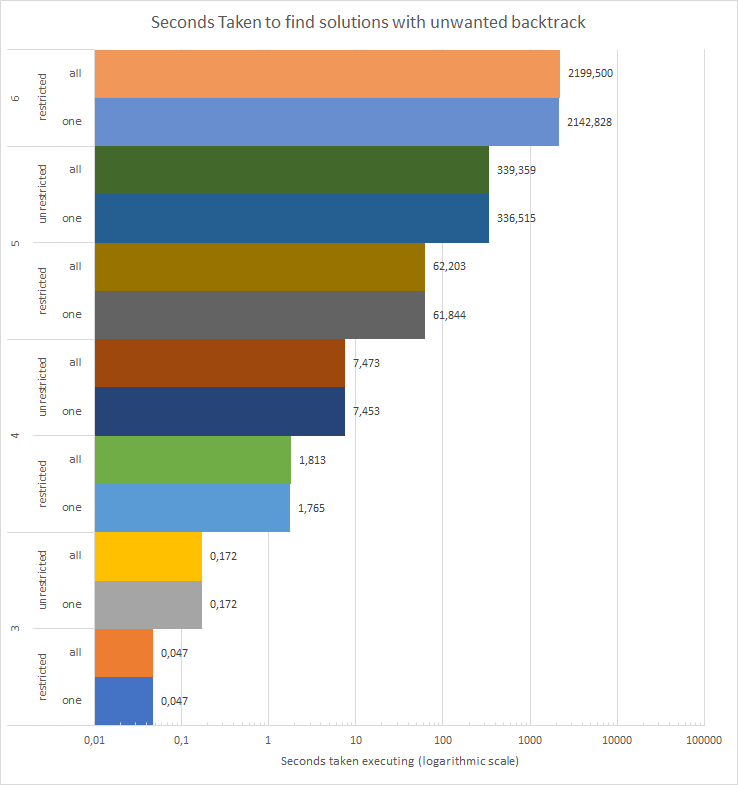
\includegraphics[width=\textwidth]{figuras/graphs/unwanted_bt.png}
\caption{Gráfico correspondente aos dados da tabela \ref{tab:unwanted_bt} com resultados de execução com backtracking indesejado}
\label{gph:without_unwanted_bt}
\end{figure}
\begin{figure}[ht]
\centering
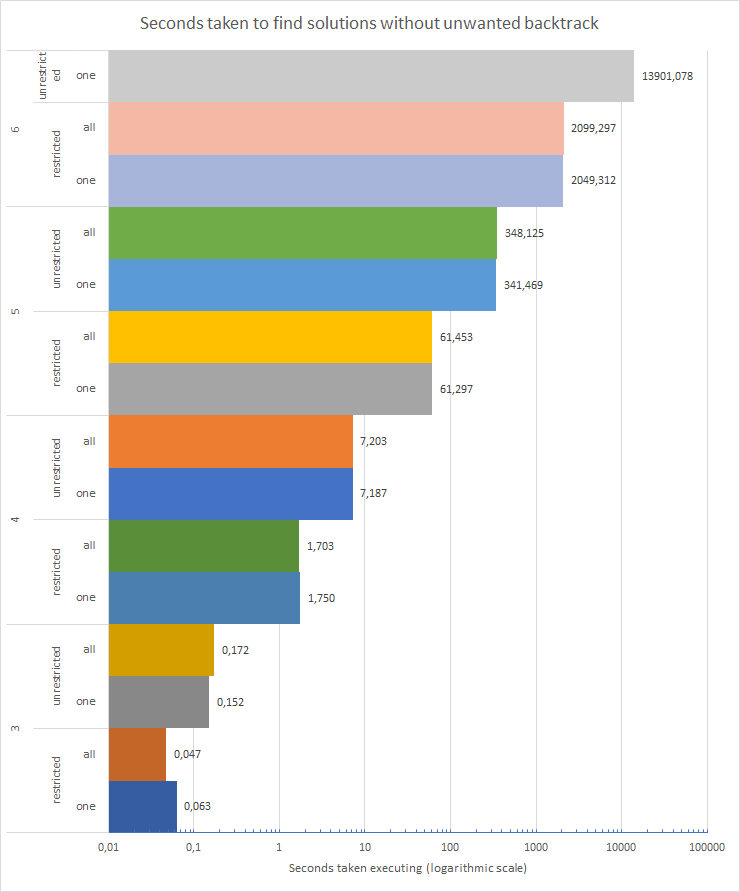
\includegraphics[width=\textwidth]{figuras/graphs/without_unwanted_bt.png}
\caption{Gráfico correspondente aos dados da tabela \ref{tab:rmv_unwanted_bt} com resultados de execução sem backtracking indesejado}
\label{gph:unwanted_bt}
\end{figure}
\begin{figure}[ht]
\centering
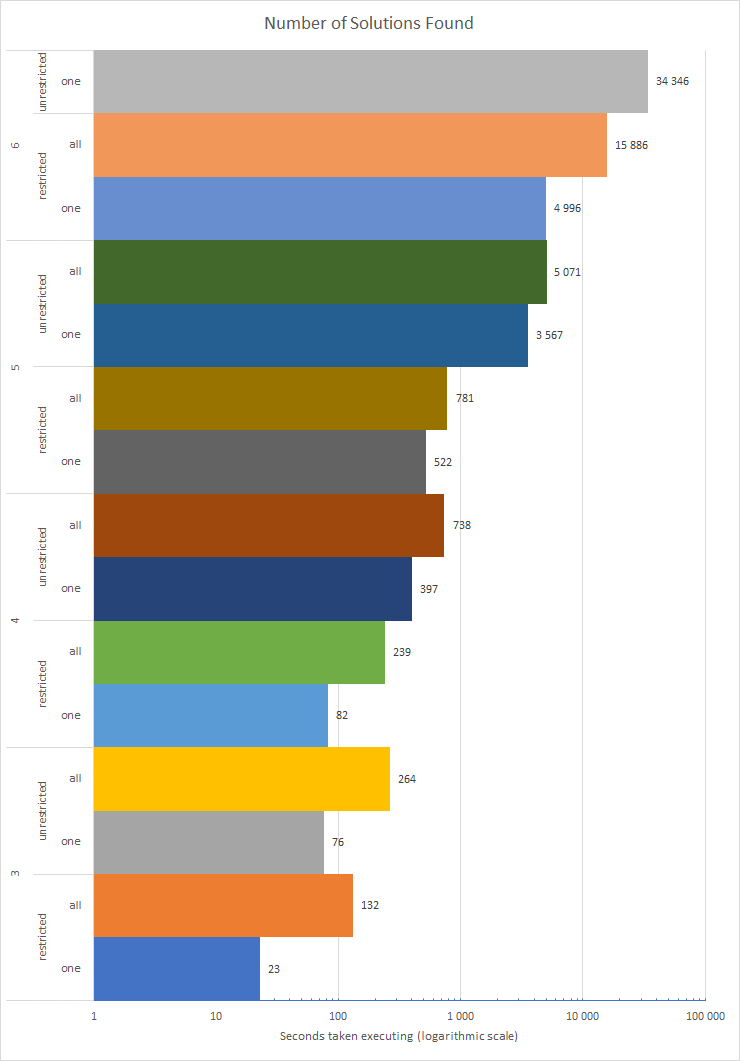
\includegraphics[width=\textwidth]{figuras/graphs/solutions.png}
\caption{Numero de soluções encontradas para cada tipo de pesquisa. Estes números são comuns a todas as experiências}
\label{gph:solutions}
\end{figure}
\begin{figure}[ht]
\centering
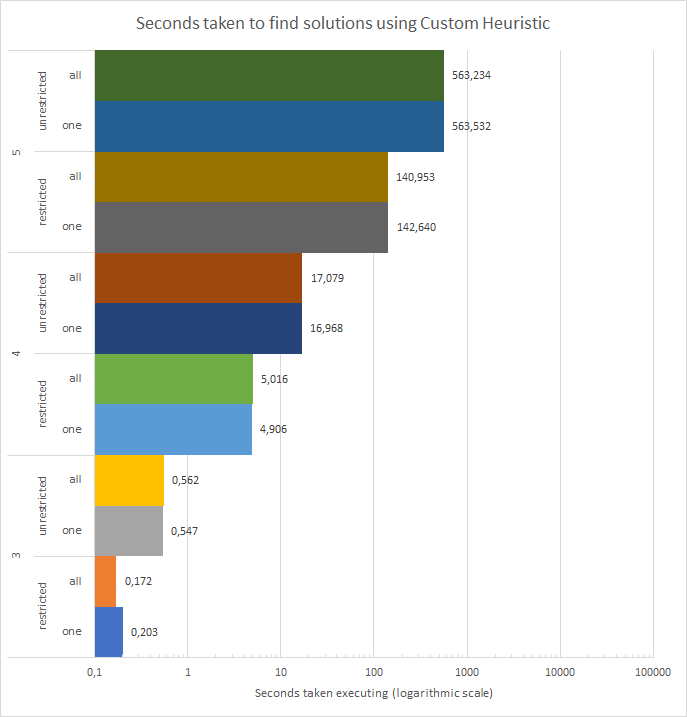
\includegraphics[width=\textwidth]{figuras/graphs/custom_heuristic.png}
\caption{Gráfico com resultados da tabela \ref{tab:custom_heuristics} correspondentes aos dados obtidos com uso de uma heurística variable(Sel)}
\label{gph:custom_heuristics}
\end{figure}
\begin{figure}[ht]
\centering
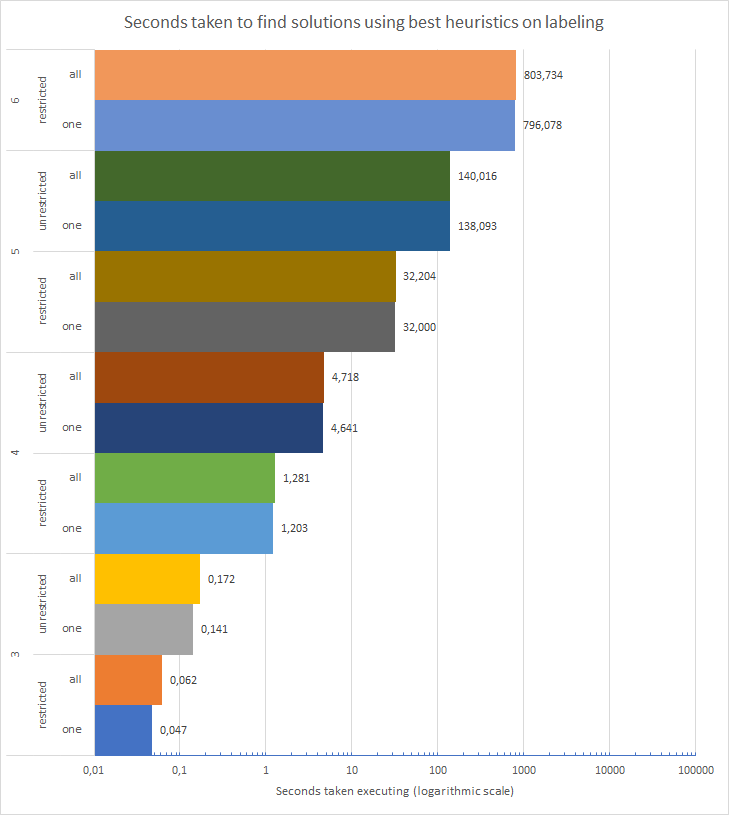
\includegraphics[width=\textwidth]{figuras/graphs/best_heuristics.png}
\caption{Gráfico com resultados da tabela \ref{tab:best_heuristics} correspondentes ao uso da melhor combinação heurística}
\label{gph:best_heuristics}
\end{figure}
\begin{figure}[ht]
\centering
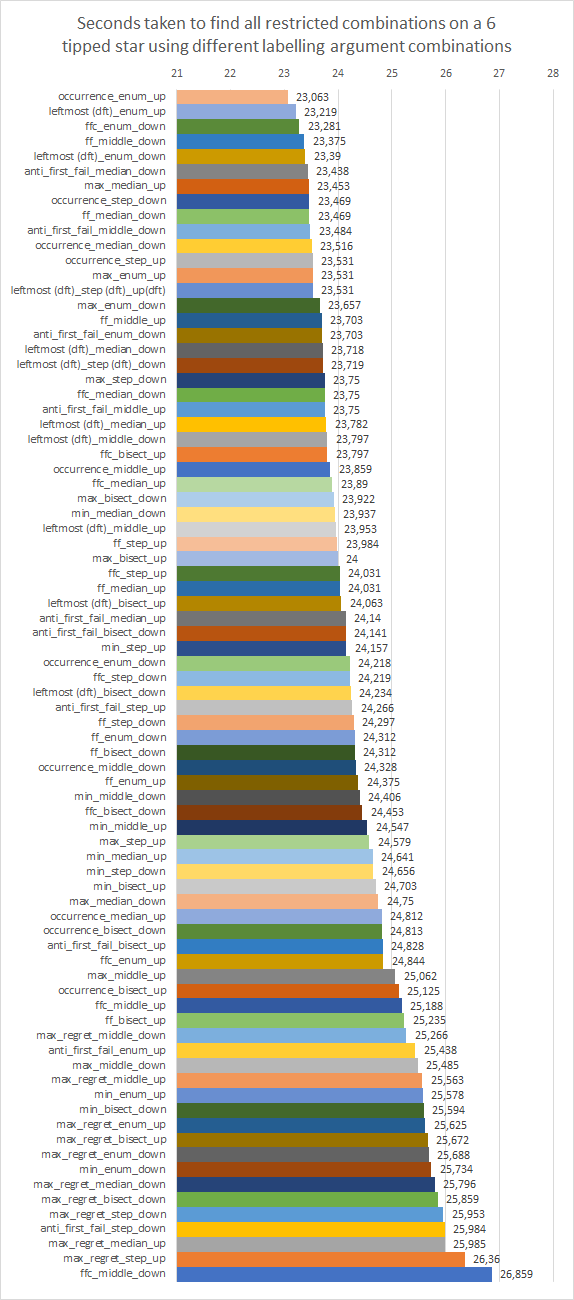
\includegraphics[width=0.75\textwidth]{figuras/graphs/ops_heuristics_analysis.png}
\caption{Resultados de teste de diferentes heurísticas no labeling de operadores}
\label{gph:ops_heuristics_analysis}
\end{figure}
\begin{figure}[ht]
\centering
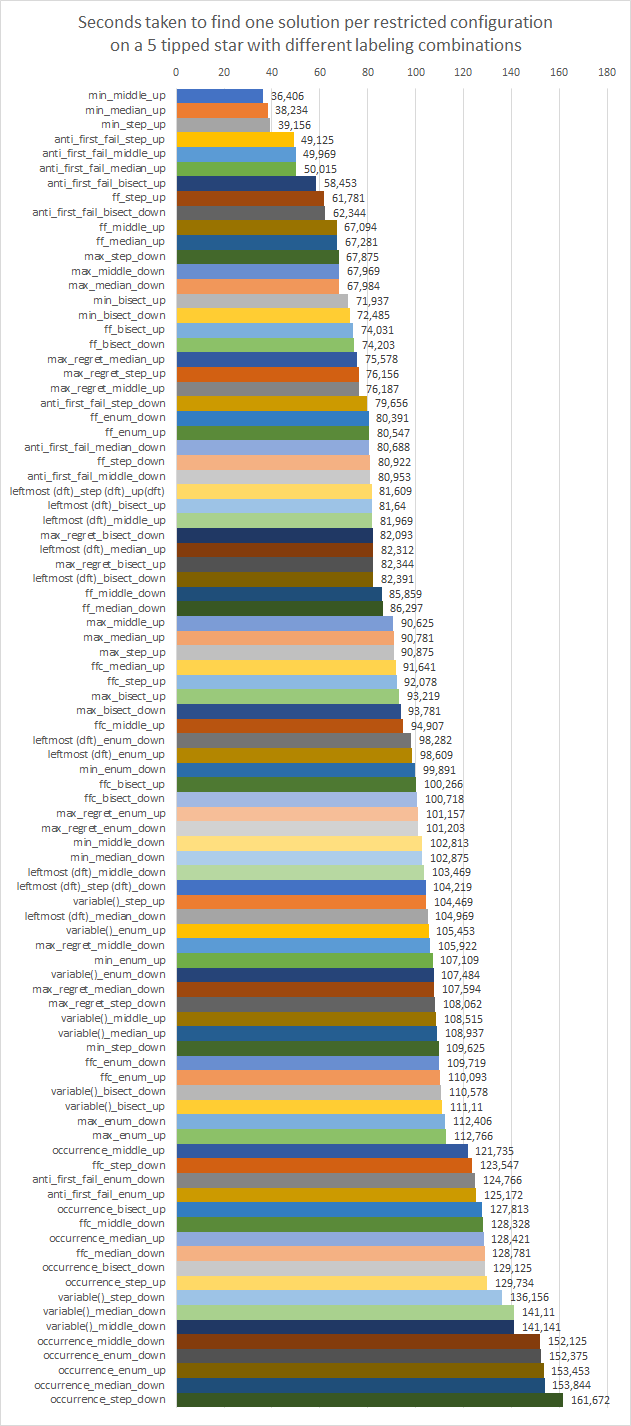
\includegraphics[width=0.75\textwidth]{figuras/graphs/solver_heuristics_analysis.png}
\caption{Resultados de teste de diferentes heurísticas no labeling da solução de puzzles}
\label{gph:solver_heuristics_analysis}
\end{figure}
\clearpage
\section{Anexos}
\begin{figure}
    \centering
    \begin{tabular}{c}
    \begin{lstlisting}[language=Prolog]
    apply_restriction(Op0i, C, A, Op7i, I, F),
    apply_restriction(Op1i, A, D, Op4i, G, J),
    apply_restriction(Op9i, B, C, Op2i, D, E),
    apply_restriction(Op8i, B, F, Op5i, H, J),
    apply_restriction(Op3i, G, E, Op6i, I, H).
    
    % predicate to apply the equation restriction
    apply_restriction(Op1, Var1, Var2, Op2, Var3, Var4):-
        apply_restriction(Op1, Var1, Var2, Value),
        apply_restriction(Op2, Var3, Var4, Value).
    apply_restriction(+, Var1, Var2, Value):-
        Var1+Var2 #= Value.
    apply_restriction(-, Var1, Var2, Value):-
        Var1-Var2 #= Value.
    apply_restriction(*, Var1, Var2, Value):-
        Var1*Var2 #= Value.
    % in case of division, the operands must be integers
    apply_restriction(/, Var1, Var2, Value):-
        % Var1/Var2 #= Value
        Var1 #= Value*Var2.
    \end{lstlisting}
    \end{tabular}
    \caption{Nas primeiras 5 linhas está uma versão desactualizada de como se estavam a definir as restrições dos operandos, usando o predicado apply\_restriction/6 fica simples aplicar as restrições a cada equação}
    \label{code:predicados_restricoes}
\end{figure}
\begin{figure}[h]
\centering
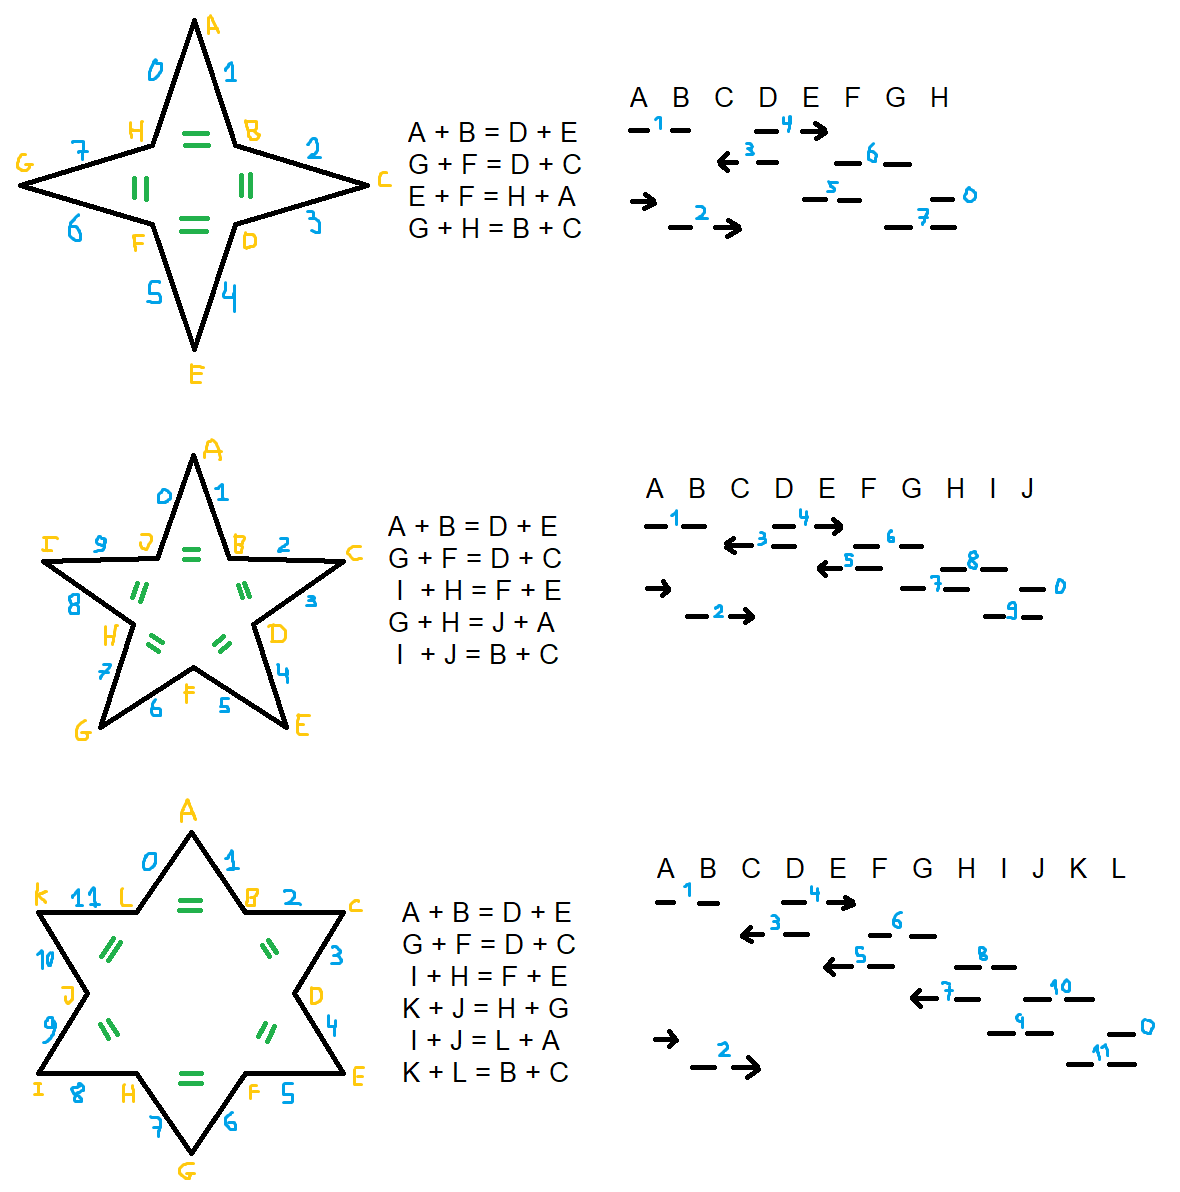
\includegraphics[width=\textwidth]{figuras/dimensional_search.png}
\caption{Método encontrado para declarar restrições de forma iterativa. Estrela de equações á esquerda, lista de equações a meio e conjunto de equações direccionais á direita}
\label{fig: restriction_method}
\end{figure}
\begin{figure}[h!]
\centering
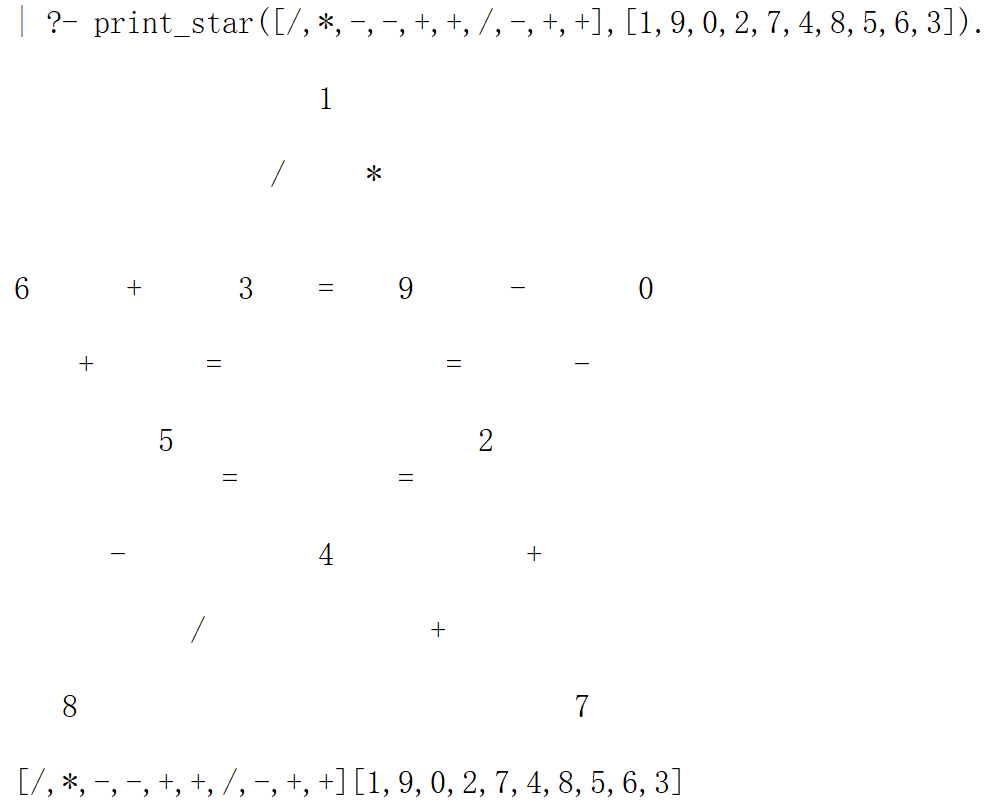
\includegraphics[width=0.5\textwidth]{figuras/representações.png}
\caption{Representação de uma estrela de 5 pontas através do predicado print\_star/2 e representação da mesma estrela em forma de listas através do predicado print\_result/2}
\label{fig: representacoes}
\end{figure}

\end{document}
